\documentclass{beamer}

\usepackage{beamerthemesplit}
\usetheme{Singapore} %Copenhagen}
%\usecolortheme{whale}

%\usepackage[T2A]{fontenc}
%\usepackage[utf8]{inputenc}
%\usepackage[russian]{babel}

\usepackage[main=russian,english]{babel}   %% загружает пакет многоязыковой вёрстки
\usepackage{fontspec}      %% подготавливает загрузку шрифтов Open Type, True Type и др.
\defaultfontfeatures{Ligatures={TeX},Renderer=Basic}  %% свойства шрифтов по умолчанию
\setmainfont{Times New Roman} %% задаёт основной шрифт документа
%\usefonttheme{professionalfonts}% SOLUTION
\usefonttheme{serif}

\usepackage{hyperref}
\usepackage{textcomp}
\usepackage{amssymb,amsmath}
%\usepackage{animate}
%\usepackage{longtable}
\usepackage{xcolor}

%\usepackage{pgffor}
\usepackage{enumitem}
\usepackage[export]{adjustbox}

\newcounter{N}

%% Форматирование окружения itemize
%\usepackage{ragged2e}
%\let\olditem\item
%\renewcommand\item{\olditem\justifying}

\usepackage{ mathrsfs }
\newcommand{\Rho}{\mathscr{P}}

\renewcommand{\Re}{\operatorname{Re}}

\newcommand{\argxi}{(\xi^1,\xi^2,\xi^3)}
\newcommand{\argx}{(x^1,x^2,x^3)}

\newcommand{\argxiv}{(\vec{\xi})}
\newcommand{\argxv}{(\vec{x})}


\newcommand{\argxbarn}{(\bar{x}^1,\bar{x}^2,\ldots, \bar{x}^n)}
\newcommand{\argxn}{(x^1, x^2,\ldots, x^n)}

\newcommand{\argtxi}{(t, \xi^1,\xi^2,\xi^3)}
\newcommand{\argtoxi}{(t_0, \xi^1,\xi^2,\xi^3)}

\newcommand{\argtxiv}{(t, \vec{\xi})}
\newcommand{\argtoxiv}{(t_0, \vec{\xi})}


\newcommand{\argtx}{(t, x^1,x^2,x^3)}
\newcommand{\argtox}{(t_0, x^1,x^2,x^3)}

\newcommand{\argtxv}{(t, \vec{x})}
\newcommand{\argtoxv}{(t_0, \vec{x})}


\newcommand{\pd}[2]{\frac{\partial #1}{\partial #2}}
\newcommand{\pdk}[2]{\frac{\partial^2 #1}{\partial #2^2}}

\newcommand{\od}[2]{\frac{d #1}{d #2}}

\newcommand{\grad}{\operatorname{grad}}
\newcommand{\rot}{\operatorname{rot}}
\newcommand{\divo}{\operatorname{div}}

\title[]{Плоские потенциальные течения идеальной жидкости. Обтекание тел.}

\author[]{ {\em Верещагин Антон Сергеевич}
\\
канд. физ.-мат. наук, старший преподаватель\\
\bigskip
Кафедра аэрофизики и газовой динамики ФФ НГУ}

\usebackgroundtemplate{
\includegraphics[width=\paperwidth]{../img/background.png}}

\begin{document}
	
\frame{\titlepage}


\frame{
	\frametitle{Аннотация}
	\parbox{\textwidth}{
		Обтекание абсолютно твёрдого тела. Задание граничных условий. Формулы Блазиуса-Чаплыгина. Формулы Кутта-Жуковского. 
	}
}

\frame{
	\frametitle{ Задача обтекания абсолютно твёрдого тела }
	
	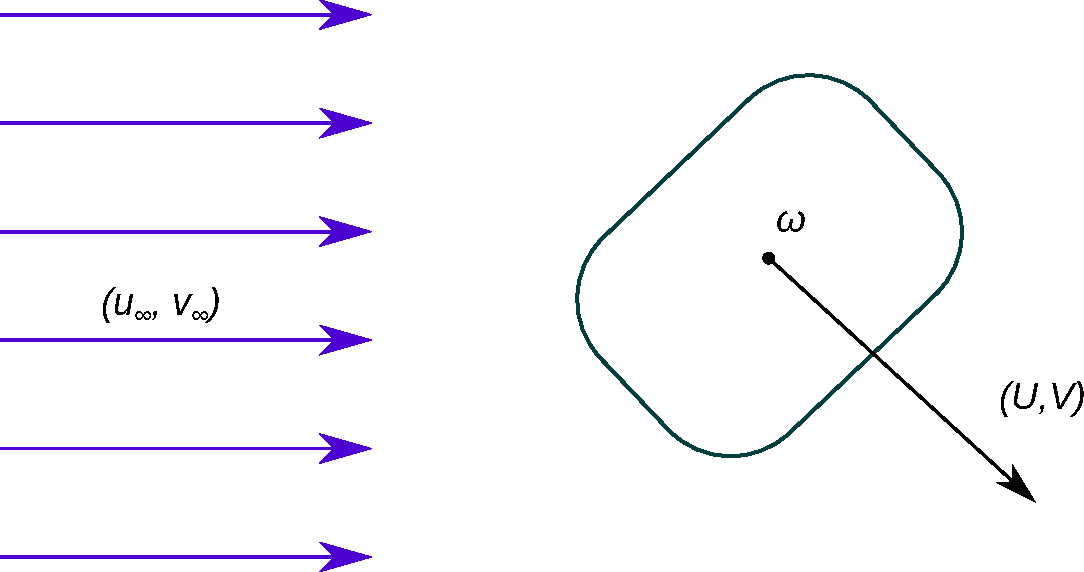
\includegraphics[width=\linewidth]{../img/flow_body.pdf}
}


\frame{
	\frametitle{ Математическая постановка задачи обтекания тела потенциальным потоком идеальной жидкости}

	\begin{exampleblock}{}
	\parbox{\textwidth}{
		Требуется найти \alert{аналитический комплексный потенциал}
		\[
			w(z) = \varphi(x,y) + i \psi(x,y),\quad
			z = x + i y,
		\]
		определённый в рассматриваемой бесконечной области, и такой что 
		\[
			\Delta \psi(x,y) = 0,
		\]
		связанный соответствующими условиями на бесконечности и границе с телом.
	}
	\end{exampleblock}

	\begin{exampleblock}{Замечание}
		\parbox{\textwidth}{
			Так как потенциал $\varphi$ связан с функцией тока $\psi$ соотношениями Коши-Римана, то функция тока находится автоматически. Можно, наоборот, искать потенциал $\varphi$, а $\psi$ выражать через соотношения Коши-Римана.
		}
	\end{exampleblock}
	
}


\frame{
	\frametitle{ Плоское покоящееся течение на бесконечности }
	
	\begin{exampleblock}{Условия на бесконечности}
		\parbox{\textwidth}{
		\[
			\pd{\psi}{x} = 0,\quad
			\pd{\psi}{y} = 0
		\]
		для бесконечно удалённых точек пространства, т.к. скорость на бесконечности равна $0$.
		}
	\end{exampleblock}
}

\frame{
	\frametitle{ Условие <<непротекания>> на границе с телом }
	
	\begin{columns}
		\begin{column}{0.4\textwidth}
			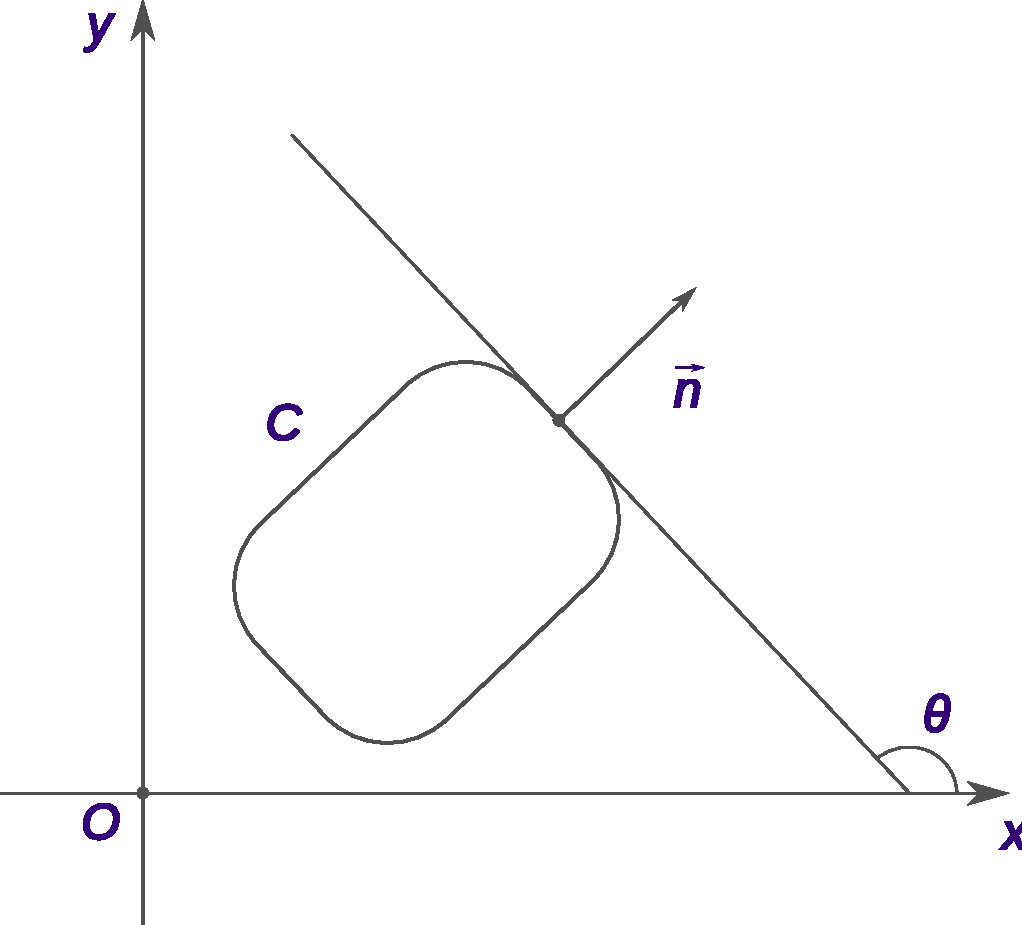
\includegraphics[width=\linewidth]{../img/vn.pdf}
		\end{column}
		\begin{column}{0.6\textwidth}
			\begin{exampleblock}{Условие на границе с телом}
				\parbox{\textwidth}{
					Нормальная составляющая (относительно границы тела) скорость течения должна совпадать с нормальной составляющей скорости тела.
				}
			\end{exampleblock}
		\end{column}
	\end{columns}

	\parbox{\textwidth}{
		\[
		v_n = v_x \cos(\vec{n},x) +v_y \cos (\vec{n},y) = v_x \sin\theta - v_y \cos\theta=
		\]
		\[
		=
		v_x\od{y}{s}-v_y\od{x}{s} = \pd{\psi}{y}\od{y}{s}+\pd{\psi}{x}\od{x}{s} = \pd{\psi}{s},
		\]
		где $x(s)$, $y(s)$ -- параметризованная граница тела в окрестности рассматриваемой точки.
	}

}

\frame{
	\frametitle{ Условие для движения абсолютно твёрдого тела}
	
	\parbox{\textwidth}{
	Пусть тело совершает поступательное движение со скоростью $(U,V)$ и вращательное с угловой скоростью $\omega$, тогда скорости точек тела будут иметь вид
	\[
	u_x = U - \omega y,\quad
	u_y = V+\omega x,
	\]
	где $(x,y)$ -- координаты точек тела во вращающейся системе координат, жёстко связанной с телом.
	}	\pause

	
	\begin{exampleblock}{Условие на границе с телом}
		\parbox{\textwidth}{
			\[
		\pd{\psi}{s} = 
		u_x \cos (\vec{n},y) + u_y \cos (\vec{n},y)	=
		u_x \od{y}{s} - u_y \od{x}{s} =
		\]
		\[
		=
		(U - \omega y)\od{y}{s} - (V+\omega x) \od{x}{s}.
		\]	
		
		Отсюда,
		\[
		\psi = U y - V x -\frac{1}{2}\omega(x^2+y^2) + c.
		\]
		}
	\end{exampleblock}
	

	
}

\frame{
	\frametitle{ Частный случай набегающего потока на покоящееся тело }
	
	\begin{exampleblock}{Условие на границе тела}
		\parbox{\textwidth}{
			В случае покоящегося тела $U=V=0$, $\omega=0$ условие на границе тела будет
			\[
				\psi(x,y) = const.
			\]
			
		}
	\end{exampleblock}

	\begin{exampleblock}{Условие на бесконечности}
		\parbox{\textwidth}{
			В случае набегающего потока с параметрами на бесконечности равными 
			\[
			v_x=v_\infty,\quad 
			v_y = 0,
			\]
			то для бесконечно удалённых точек
			\[
			\psi(x,y) = v_\infty y + const.
			\]
		}
	\end{exampleblock}
	
}

\frame{
	\frametitle{ Задача обтекание тела }
	
		\parbox{\textwidth}{
			Таким образом, задача обтекания тела плоским потенциальным потоком идеальной жидкости сводится к решению \alert{задачи Дирихле} для функции тока $\psi$: 
			\begin{itemize}[label=\textbullet]
				\item
			внутри исследуемой области решается уравнение Лапласа 
			\[
			\Delta \psi = 0, 
			\]
			\item
			а на бесконечности и границе обтекаемого тела заданы значения функции $\psi$ в зависимости от условий обтекания.
			\end{itemize}
			
			
		}
	
}

\frame{
	\frametitle{ Сила  при безотрывном обтекании }
	
	\begin{exampleblock}{Определение}
		\parbox{\textwidth}{
			По аналогии с комплексными скоростью и потенциалом, определим комплексную силу $R$, действующую на контур $C$ в области течения по формуле
			\[
			R = X + i Y,
			\]
			где $X$, $Y$ -- вещественные проекции силы на оси координат.
			
		}
	\end{exampleblock}	
}

\frame{
	\frametitle{ Формула для силы через давление при безотрывном обтекании}
	
	\centering
	\begin{columns}
		\begin{column}{0.5\textwidth}
			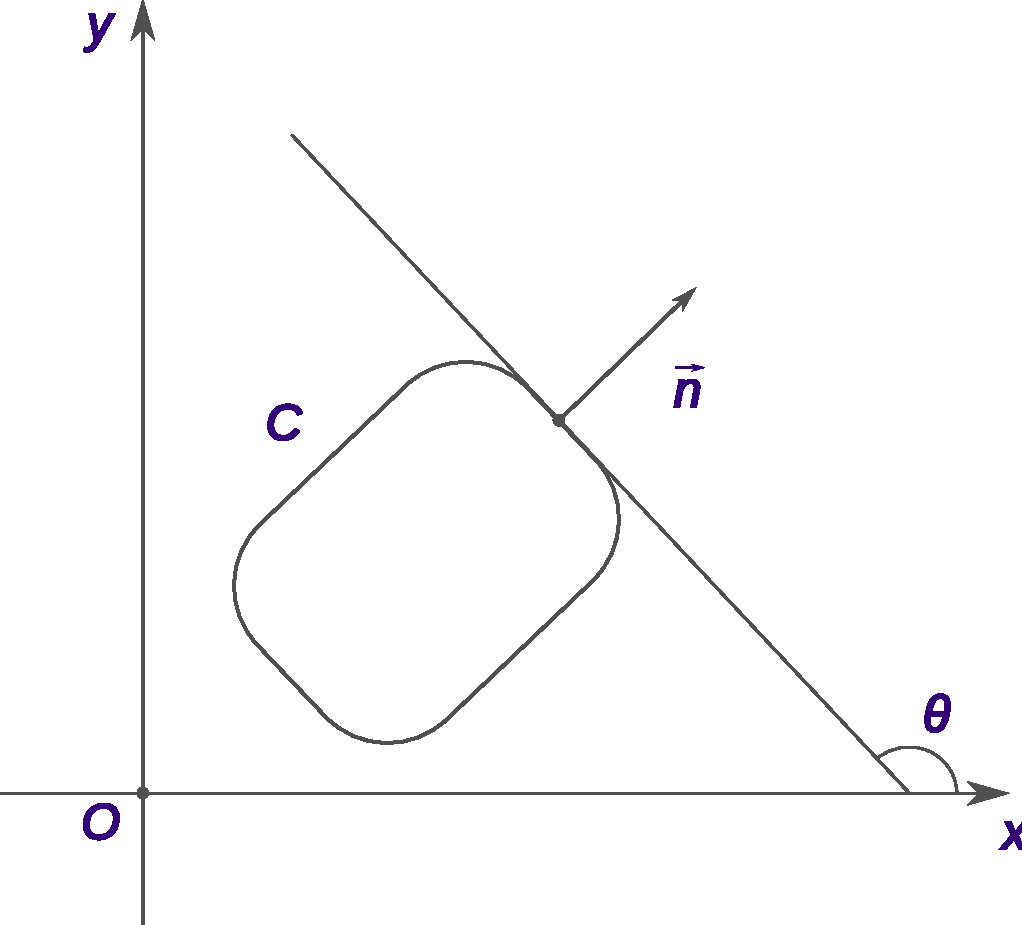
\includegraphics[width=\linewidth]{../img/vn.pdf}
		\end{column}
		\begin{column}{0.5\textwidth}
			\begin{exampleblock}{}
				\parbox{\textwidth}{
					Комплексно-сопряжённая сила $R^*$ вдоль контура тела $C$ при безотрывном обтекании
					\[
					R^* = X - i Y = 
					\]
					\[
					=
					-\oint\limits_C p (\cos(\vec{n},x) - i \cos(\vec{n},y)) ds = 
					\]
					\[
					=
					-\oint\limits_C p (\sin\theta + i \cos\theta) ds = 
					\]
					\[
					=
					-i \oint\limits_C p e^{-\theta i} ds.
					\]
					
					
				}
			\end{exampleblock}
		\end{column}
	\end{columns}
		

}

\frame{
	\frametitle{ Предварительные выкладки }
	
	\begin{exampleblock}{Выражение для комплексного дифференциала}
		\parbox{\textwidth}{
			\[
			dz = dx + i dy = ds(\cos\theta + i \sin\theta) = e^{i\theta}ds,
			\]
			\[
			dz^* = dx - i dy = ds(\cos\theta - i \sin\theta) = e^{-i\theta}ds.
			\]
			Отсюда
			\[
			dz^* = e^{-2\theta i} dz.
			\]
			
		}
	\end{exampleblock}\pause

	\begin{exampleblock}{Интеграл Бернулли}
		\parbox{\textwidth}{
			Связь давления и скорости через интеграл Бернулли
			\[
				p = c - \frac{1}{2}\rho v^2
			\]
			справедлива вдоль контура тела при безотрывном обтекании, т.к. он является линией тока. При потенциальном течении она справедлива во всей области течения.
			
		}
	\end{exampleblock}

	
}


\frame{
	\frametitle{ Сила }
	
	
	\begin{exampleblock}{}
		\parbox{\textwidth}{
		\[
			R^* = -i c \oint\limits_{C}d z^* + \frac{i \rho}{2} \oint\limits_C v^2 dz^*=
			\frac{i \rho}{2} \oint\limits_C v^2 dz^*=
			\frac{i \rho}{2} \oint\limits_C (v e^{-i \theta})^2 dz.
		\]\pause
		
		Используя то, что
		\[
		v e^{-i \theta} = v \cos\theta -i v \sin\theta = v_x-i v_y = v^*,
		\]
		получим 
		\[
		R^* = X - i Y = \frac{i\rho}{2} \oint\limits_C (v^*)^2 dz.
%		 = \frac{i\rho}{2} \oint\limits_C \left(\od{w}{z} \right)^2 dz
		\]
		
		}
	\end{exampleblock}
}

\frame{
	\frametitle{ Момент главных сил }
	\parbox{\textwidth}{
	\[
	L = -\oint\limits_C p (x \cos(\vec{n},y)-y\cos(\vec{n},x)) ds =
	-\oint\limits_C p (x \cos\theta + y\sin\theta) ds =
	\]
	\[
	=
	-\oint\limits_C p (x dx + y dy) =
		-\oint\limits_C \left(c + \frac{\rho v^2}{2}\right) (x dx + y dy) =
	\]
	\[
	=
	-\oint\limits_C c\, d(x^2+y^2) - \frac{\rho}{2}\oint\limits_C v^2 (x dx + y dy)=
%	\]
%	\[
%	= 
	\Re \left( 
	-\frac{\rho}{2}\oint\limits_C v^2zdz^*
	\right)=
	\]
	\[
	=
	\Re \left( 
	-\frac{\rho}{2}\oint\limits_C (v^*)^2zdz,
	\right),
	\]
	т.к. $v^2 dz^* = (v^*)^2 dz$.
	}
	
}

\frame{
	\frametitle{ Формулы Блазиуса-Чаплыгина для потенциального течения }
	
	\begin{exampleblock}{ }
		\parbox{\textwidth}{
			Если течение потенциально, тогда существует комплексный потенциал
			\[
			w(z)= \varphi(z) + i \psi(z) \quad\text{и}\quad
			\od{w}{z} = v^*.
			\]
		}
	\end{exampleblock}

	\begin{exampleblock}{ Формулы Блазиуса-Чаплыгина }
		\parbox{\textwidth}{
		\[
		R^* = X - i Y = \frac{i\rho}{2} \oint\limits_C \left(\od{w}{z} \right)^2 dz,
		\]	
		\[
		L = \Re \left[
		-\frac{\rho}{2}\oint\limits_C \left(\od{w}{z} \right)^2 zdz
		\right].
		\]
		}
	\end{exampleblock}
}

\frame{
	\frametitle{ Формула Кутта-Жуковского }

\begin{exampleblock}{Предположения }
	\parbox{\textwidth}{
		Поток потенциален везде вне тела, которое можно заменить на конечное число источников, вихрей и диполей, лежащих внутри границы тела, контура $C$.
	}
\end{exampleblock}


\begin{exampleblock}{Формула для силы и реакции}
	\parbox{\textwidth}{
		\[
		R^* =  X - iY = i\rho\Gamma v_\infty^*,		
		\]
		\[
		L = \Re \left[
		-\rho v_\infty^*\sum\limits_{k=1}^m\Gamma_kb_k-i\rho M v_\infty^*
		\right],
		\]
		где
		$\Gamma_i$ -- циркуляции вихрей, находящихся в точках $b_i$ $(i=1,\ldots,m)$; $M$ -- суммарный момент источников и диполей, $\Gamma$ -- суммарная циркуляция вихрей, находящихся внутри тела.
	}
\end{exampleblock}

}




\frame{
	\frametitle{ Литература }
	\begin{itemize}[partopsep=1pt,label=\textbullet]
		\item 
		{\em Кочин~Н.~Е., Кибель~И.~А., Розе~Н.~В.} Теоретическая гидромеханика. М.:Гос. издат. физ.-мат. лит., 1963.
	\end{itemize}
}

\end{document}